\documentclass[10pt, a4paper]{article}
\usepackage[utf8]{inputenc}
\usepackage[paper=a4paper, left=1.5cm, right=1.5cm, bottom=1.5cm, top=3.5cm]{geometry}
\usepackage[spanish]{babel}
\usepackage{indentfirst}
\usepackage{fancyhdr}
\usepackage{latexsym}
\usepackage{lastpage}
\usepackage[colorlinks=true, linkcolor=blue]{hyperref}
\usepackage{calc}
\usepackage{verbatim}
\usepackage{listings}
\usepackage{amsfonts}
\usepackage{float}
\setcounter{tocdepth}{5}
\usepackage{caption}
\usepackage{subcaption}
\sloppy

\parskip=5pt % 10pt es el tamaño de fuente

% Pongo en 0 la distancia extra entre ítemes.
\let\olditemize\itemize
\def\itemize{\olditemize\itemsep=0pt}

\usepackage{caratula}

% Acomodo fancyhdr.
\pagestyle{fancy}
\thispagestyle{fancy}
\addtolength{\headheight}{1pt}
\lhead{S. Aboy Solanes, E. Almansi, F. Canay, F. Decroix}
\rhead{$2^{\mathrm{do}}$ cuatrimestre de 2014}
\cfoot{\thepage /\pageref{LastPage}}
\rfoot{Trabajo Práctico 1 - Wiretapping}
\renewcommand{\footrulewidth}{0.4pt}

\begin{document}


\titulo{Trabajo Práctico 1 - Wiretapping}
\fecha{Martes 23 de Septiembre}
\materia{Teoría de las Comunicaciones}
\integrante{Santiago Aboy Solanes}{175/12}{santiaboy2@hotmail.com}
\integrante{Emilio Almansi}{674/12}{ealmansi@gmail.com}
\integrante{Federico Canay}{250/12}{fcanay@hotmail.com}
\integrante{Facundo Decroix}{842/11}{fndecroix92@hotmail.com}

%Pagina de titulo e indice
\thispagestyle{empty}

\maketitle

%\thispagestyle{empty}
%\mbox{}
%\newpage
\thispagestyle{empty}
\tableofcontents

\newpage

\section{Introducción}
En este trabajo práctico vamos a abordar el desarrollo de herramientas de diagnóstico de red. Nuestro objetivo va a ser analizar estadísticamente el protocolo ARP. Por otro lado, vamos a sacar conclusiones acerca de los tipos de dispositivos de red que se pueden encontrar en un segumento de red determinado. Para ello, utilizamos la herramienta de manipulación y análisis de paquetes, Scapy.

\section{Desarrollo}
Antes de comenzar el desarrollo vamos a definir algunos términos.

$\bullet$ \textbf{Informacion}: Dado un evento E decimos que cuando E tiene lugar, recibimos
\begin{center}
$I (E) = log(\frac{1}{P(E)})$ 
\end{center}

unidades de información. Al usar $log_2$ la unidad obtenida es bits.

$\bullet$ \textbf{Entropía}: La entropía de un mensaje X, que se representa por H(X), es el valor medio ponderado de la cantidad de información de los diversos estados del mensaje 

\begin{center}
$H(X) = - \Sigma$ $p(x)$ $log$ $p(x)$
\end{center}

$\bullet$ \textbf{Nodo distinguido}: En una fuente, un nodo distinguido es un nodo cuya información es menor a la entropía de dicha fuente.

\subsection{Capturando tráfico}
Para el desarrollo de este trabajo práctico escuchamos pasivamente redes para poder observar que sucedía en las mismas. En particular, capturamos paquetes ARP \emph{who-has}.

Utilizamos dos modelos de fuente de información:

$S_{dst}$ = \{$s_1$ $\cdots$ $s_n$\} siendo $s_i$ una IP que aparece como dirección destino en los paquetes ARP \emph{who-has}

$S_{src}$ = \{$s_1$ $\cdots$ $s_n$\} siendo $s_i$ una IP que aparece como dirección origen en los paquetes ARP \emph{who-has}

Creamos una \emph{tool} que escucha pasivamente en la red local. Luego, la adaptamos para que estime las probabilidades de dichas fuentes en función de los paquetes ARP observados y que calcule la entropía de las mismas.

Usando dicha herramienta, realizamos capturas de paquetes ARP sobre distintas LANs: Alto Palermo, Red laboral de Honeywell, Laboratorios de Ciudad Universitaria (Via Wi-Fi), y la casa de un integrante del grupo.

\subsection{Gráficos}

Una vez que capturamos el tráfico, nos propusimos gráficar y a analizar los datos obtenidos. Realizamos tres tipos de gráficos:

$\bullet$ Grafos dirigidos:
  En los grafos, los nodos son los IPs que aparecen en alguno de los paquetes capturados.
  Una arista entre A y B significa que se encontro un paquete con \emph{src} A y \emph{dst} B. El peso de cada arista corresponde a la cantidad de paquetes de la forma anterior.
  
  Ejemplo:
  
  \begin{figure}[H]
  \begin{center}
    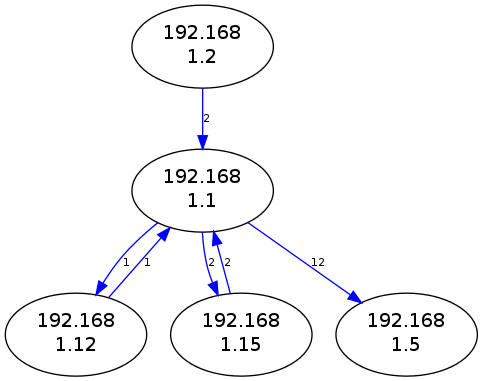
\includegraphics[width=\linewidth/2]{../imgs/pruebaFede-ips_red.png}
    \label{fig:FedeGrafo}
    \caption{Grafo de LAN hogareña}
  \end{center}
\end{figure}

$\bullet$ Histograma:
  Realizamos para cada una de las fuentes (\emph{src} y \emph{dst}), realizamos un histograma que muestra la cantidad de apariciones de un determinado IP en la fuente.
  
  Ejemplo:
  
  \begin{figure}[H]
  \begin{center}
    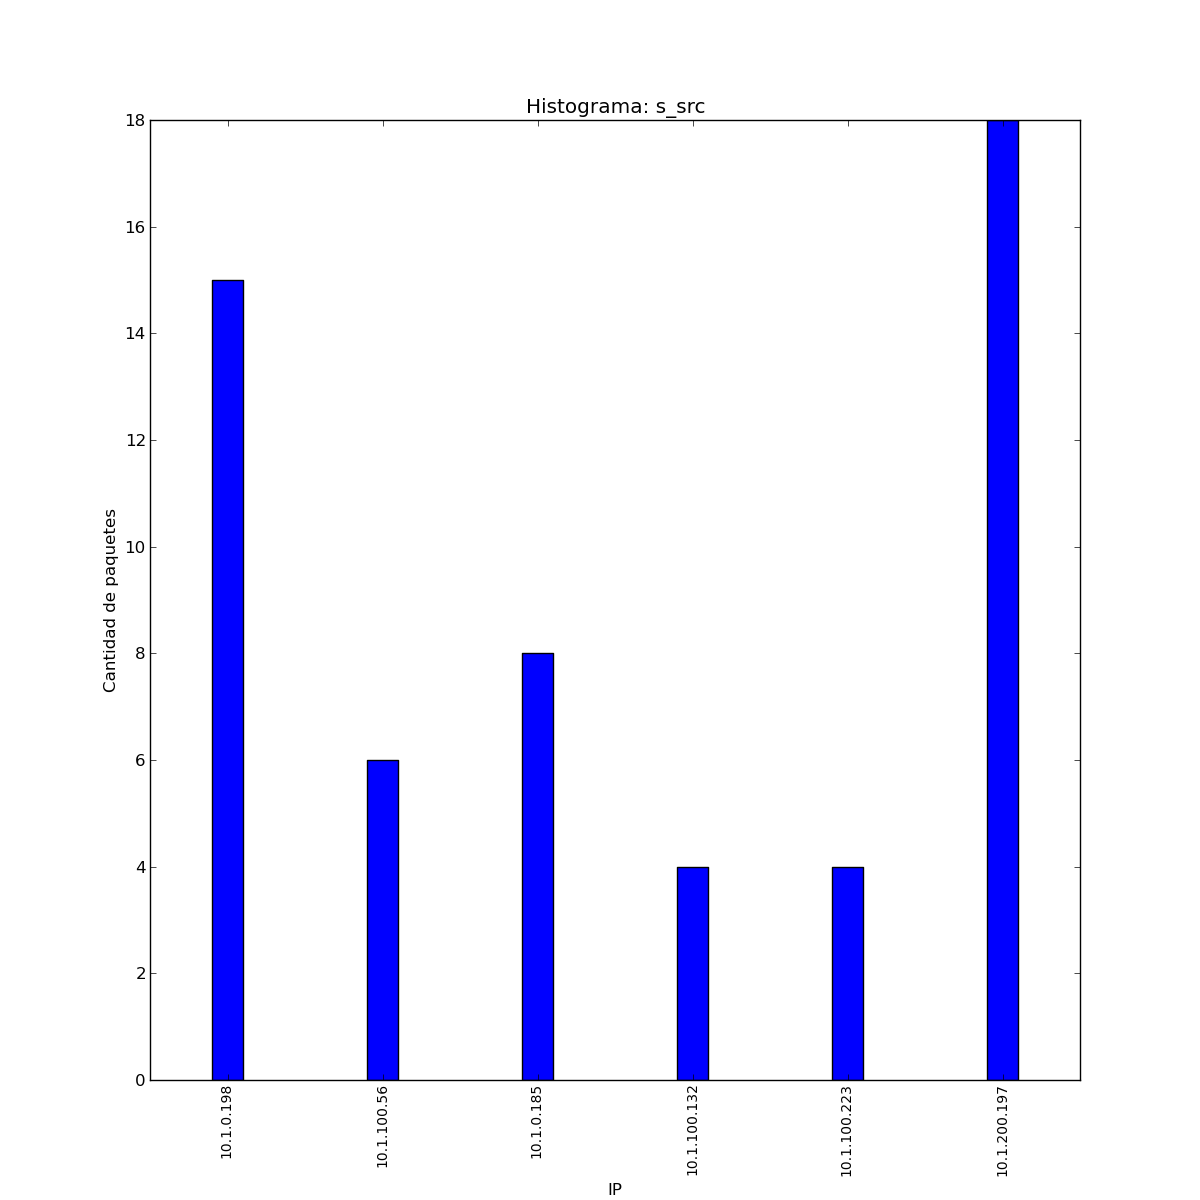
\includegraphics[width=\linewidth/2]{../imgs/entrepiso-dc-ips_s_src_hist.png}
    \caption{Histograma de la serie de paquetes s\_src de la red \emph{Entrepiso-DC}.}
    \label{fig:histograma-entrepiso-dc-s-src}
  \end{center}
  \end{figure}
  
$\bullet$ Gráfico Información:
  Realizamos para cada una de las fuentes (\emph{src} y \emph{dst}), realizamos un gráfico donde se muestra la información de un determinado IP en la fuente. Además graficamos una recta con el valor de la entropía para comparar facilmente la información de cada IP con la entropía de la fuente. 
  
  Ejemplo:
  
  \begin{figure}  
  \begin{center}
    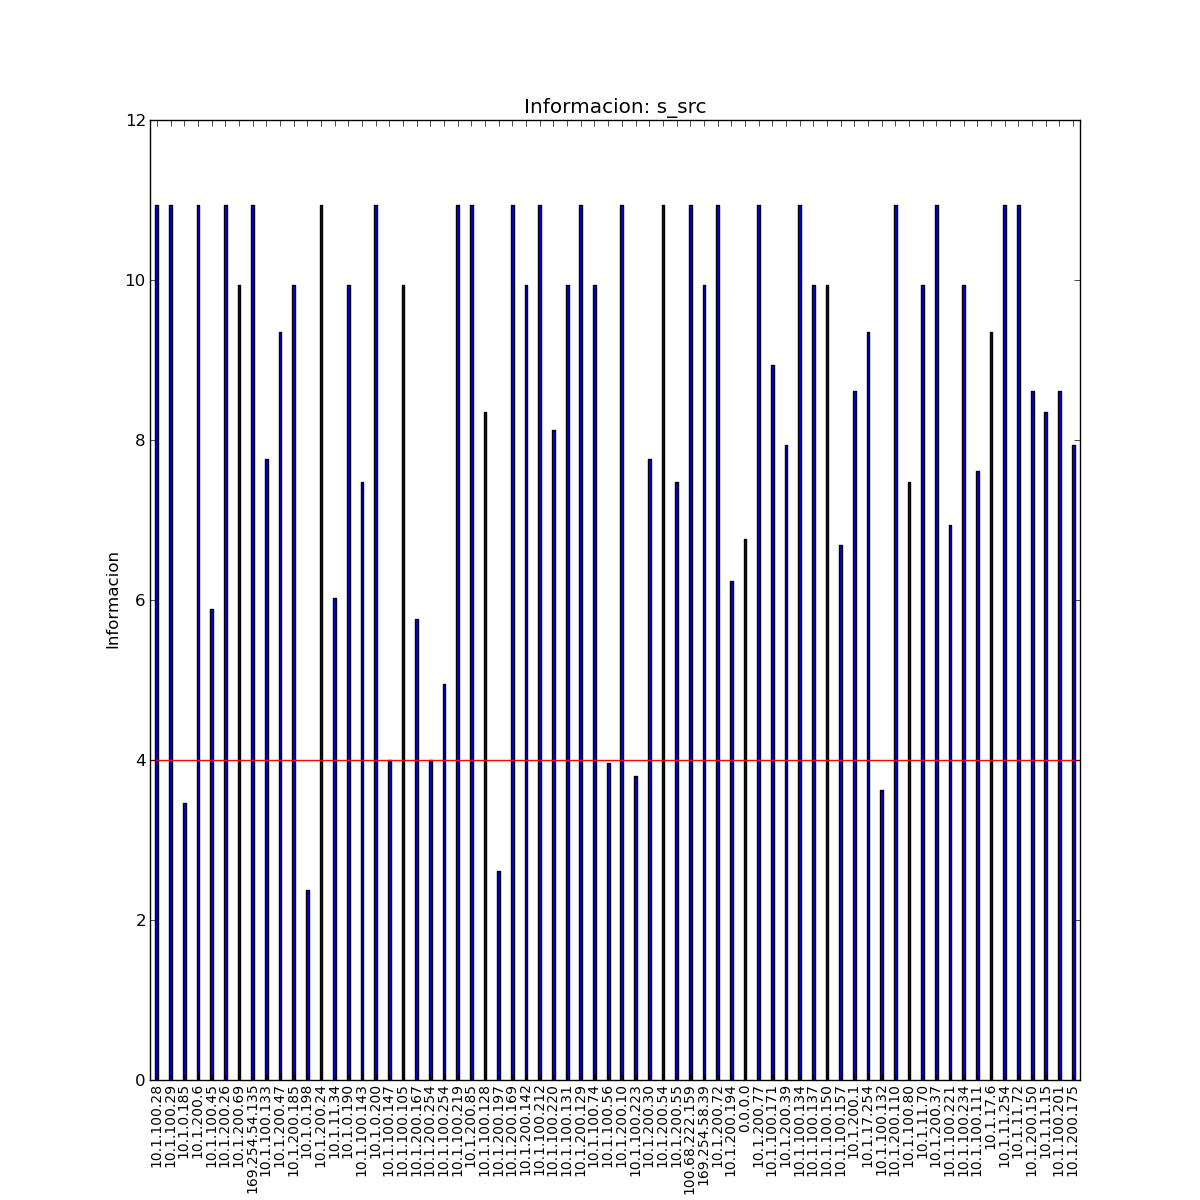
\includegraphics[width=\linewidth/2]{../imgs/entrepiso-dc-ips_s_src_info.png}
    \caption{Gráfico de cantidad de información para cada IP s\_src de la red \emph{Entrepiso-DC}.}
    \label{fig:informacion-entrepiso-dc-s-src}
  \end{center}
\end{figure}
  
Graficamos en forma de histogramas, y de grafos la información y entropía de $S_{dst}$ y $S_{src}$

\section{Resultados}

\subsection{Red Alto Palermo}

\subsubsection{Descripción y topología de la red}

lugar, dia de la semana, hora aproximada, fecha, wifi o ethernet
cantidad de paquetes tomados, tiempo de muestreo

Nuestro primer experimento consistió en medir la LAN Wi-Fi pública del shopping Alto Palermo. Esta medición se llevó a cabo el Sábado 20 de Septiembre a las 21hs, el tiempo de medición fue de aproximádamente 40 minutos y se capturaron 1569 paquetes ARP.


\subsubsection{Topología de la red}

A continuación mostramos un grafo que muestra los nodos de la red con su dirección IP y la cantidad de mensajes de tipo \emph{who-has}.

\begin{figure}
 \begin{center}
  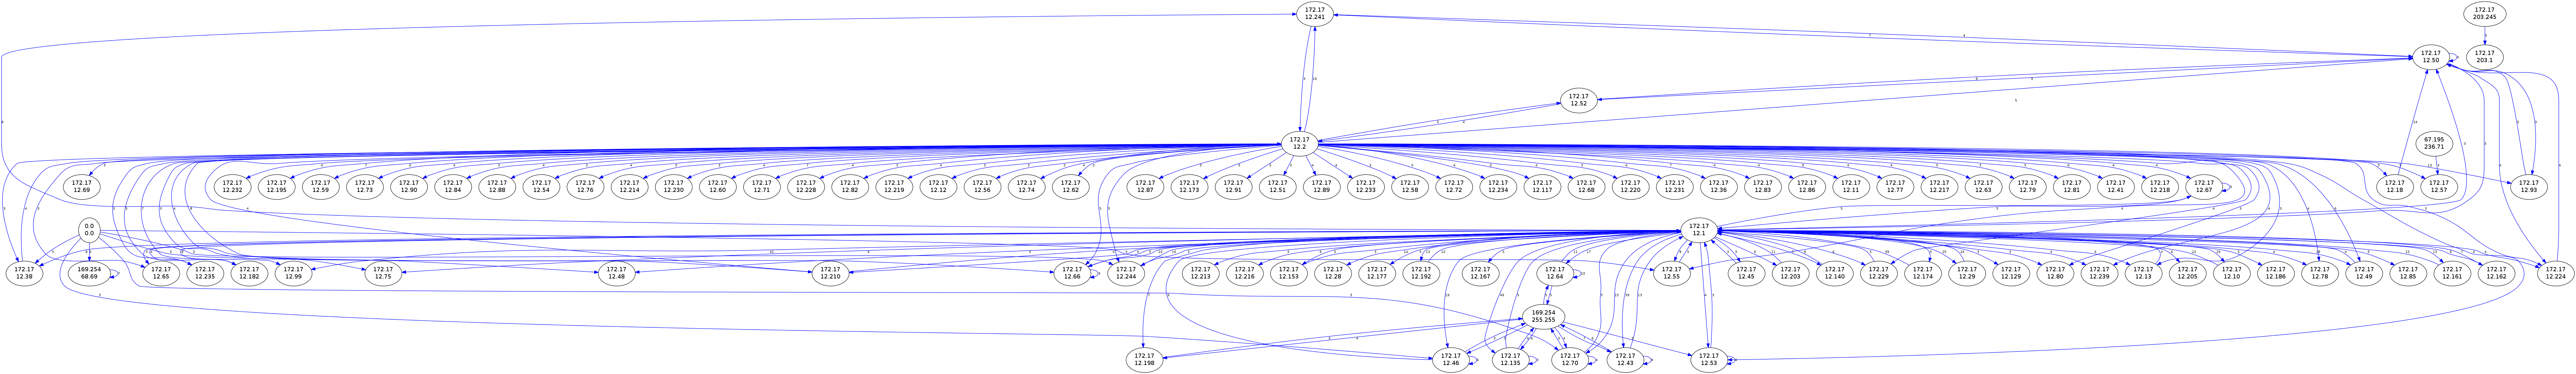
\includegraphics[width=\linewidth/2]{../imgs/snifAlto-ips_red.png}
  \caption{Grafo Medición Alto Palermo}
 \end{center}

\end{figure}

Como podemos ver en el grafo, la red tiene un nodo distinguido. Este nodo, el cual tiene la dirección IP 117.17.12.1, recibe muchos mensajes de la mayoría de los otros nodos de la red, pero no envía ninguno. Suponemos que este nodo es el router de la red.

\subsubsection{Fuente: $S_{dst}$}

A contincuación mostramos los gráficos 

\subsubsection{Fuente: $S_{src}$}

histograma
grafico de informacion
entropía total

\subsubsection{Discusión}

cualquier cosa interesante sobre este caso en particular

\subsection{Red Honeywell}

\subsubsection{Descripción y topología de la red}


lugar, dia de la semana, hora aproximada, fecha, wifi o ethernet
cantidad de paquetes tomados, tiempo de muestreo

Nuestro segundo experimento consistió en capturar los paquetes de la LAN Wi-Fi de la empresa Honeywell. En esta red no hay mucho tráfico, ya que la mayoría de las computadores se conectan via Ethernet a una VPN. Esta red es dedicada a transacciones que no necesiten un nivel de seguridad. La captura se realizo un día lunes a las 11 am. durante media hora, lográndose capturar 253 paquetes.	

\subsubsection{Topología de la red}

grafico del grafo de la red

\begin{figure}[H]
 \begin{center}
  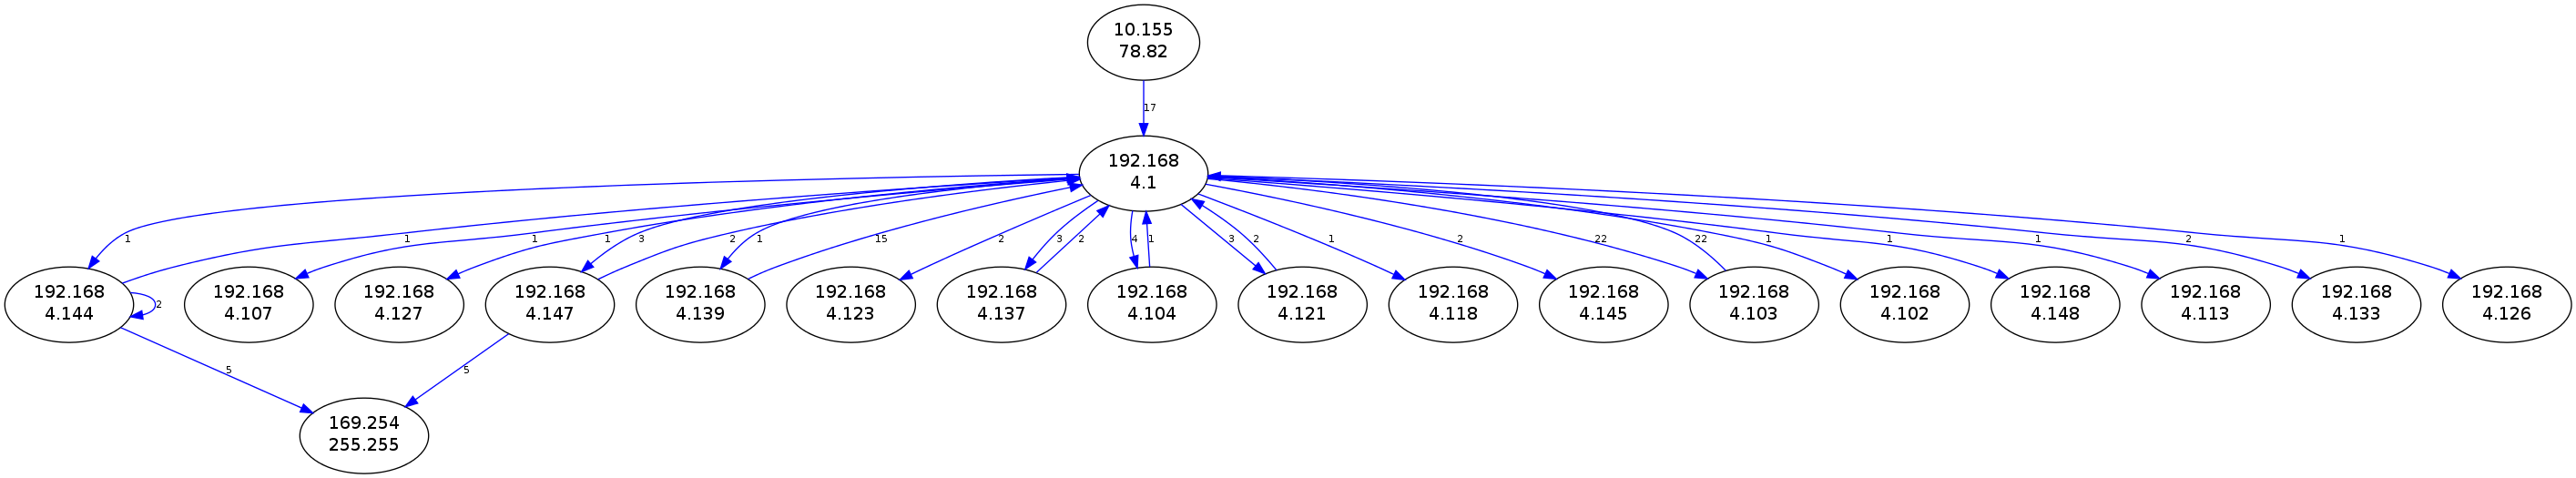
\includegraphics[width=\linewidth]{../imgs/prueba_laburo-ips_red.png}
  \caption{Medición Honeywell}
 \end{center}
\end{figure}


\subsubsection{Fuente: $S_{dst}$}

\begin{figure}[H]
   \begin{minipage}{0.5\linewidth}
     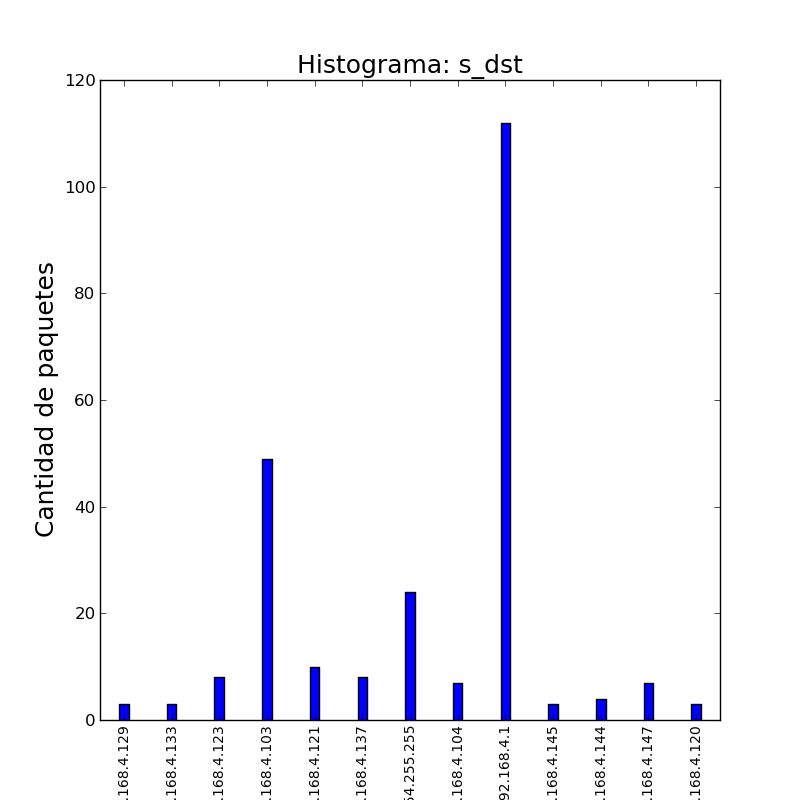
\includegraphics[width=\linewidth]{../imgs/prueba_laburo-ips_s_dst_hist.png}
     \caption{Medición Honeywell}\label{fig:Honeywell-dst-hist}
   \end{minipage}
  \hfill
   \begin{minipage}{0.5\linewidth}
     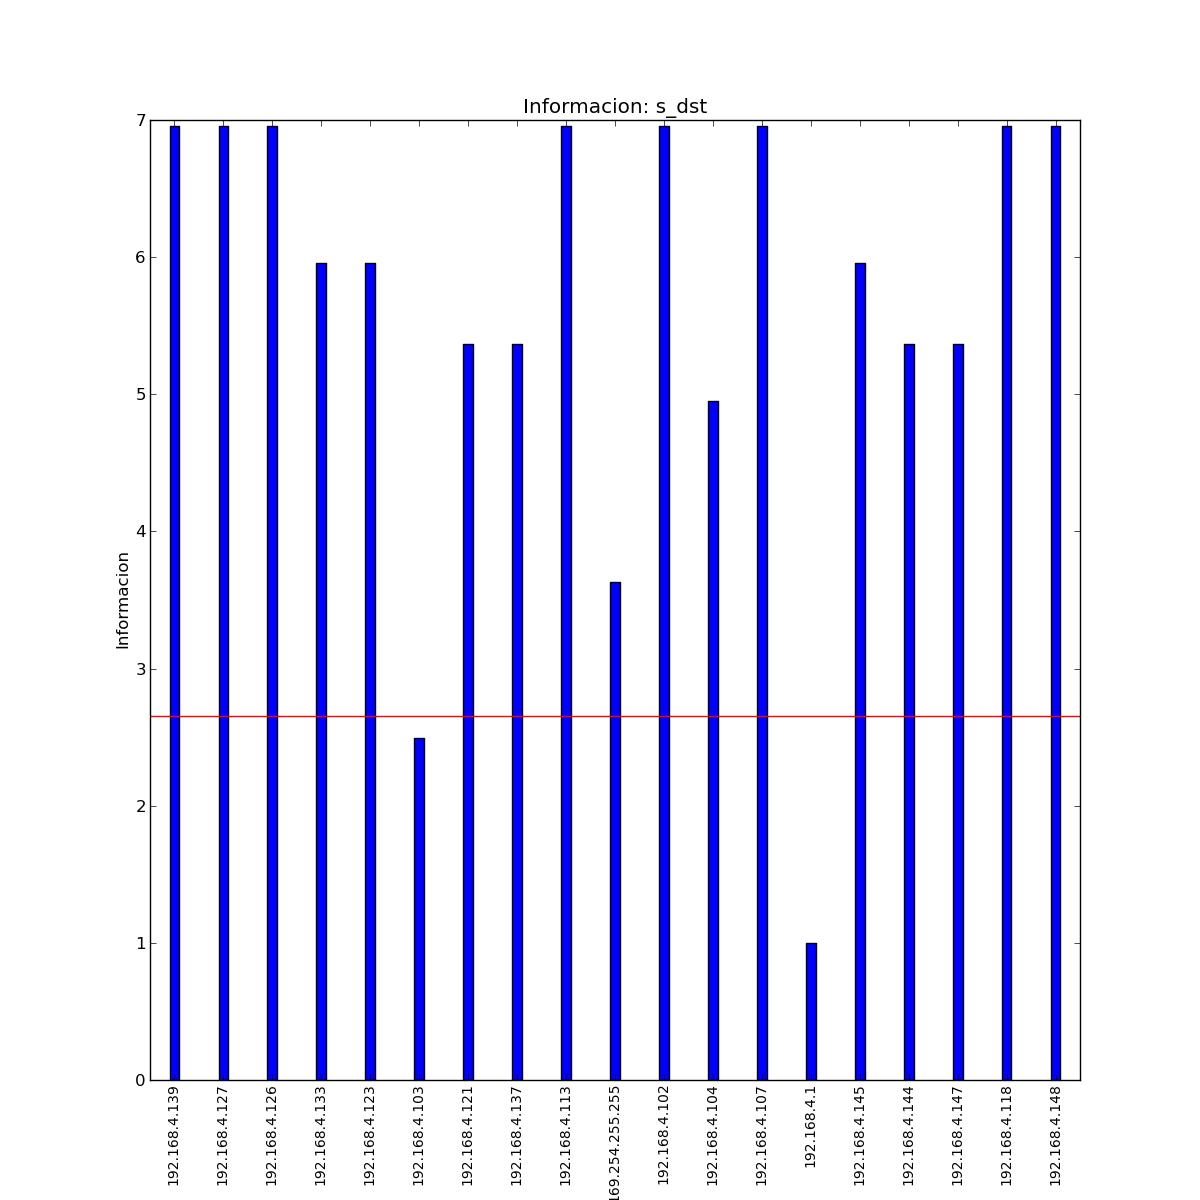
\includegraphics[width=\linewidth]{../imgs/prueba_laburo-ips_s_dst_info.png}
     \caption{Medición Honeywell}\label{fig:Honeywell-dst-info}
   \end{minipage}
 \end{figure}

histograma
grafico de informacion
entropía total

\subsubsection{Fuente: $S_{src}$}

histograma
grafico de informacion
entropía total

\begin{figure}[H]
   \begin{minipage}{0.5\linewidth}
     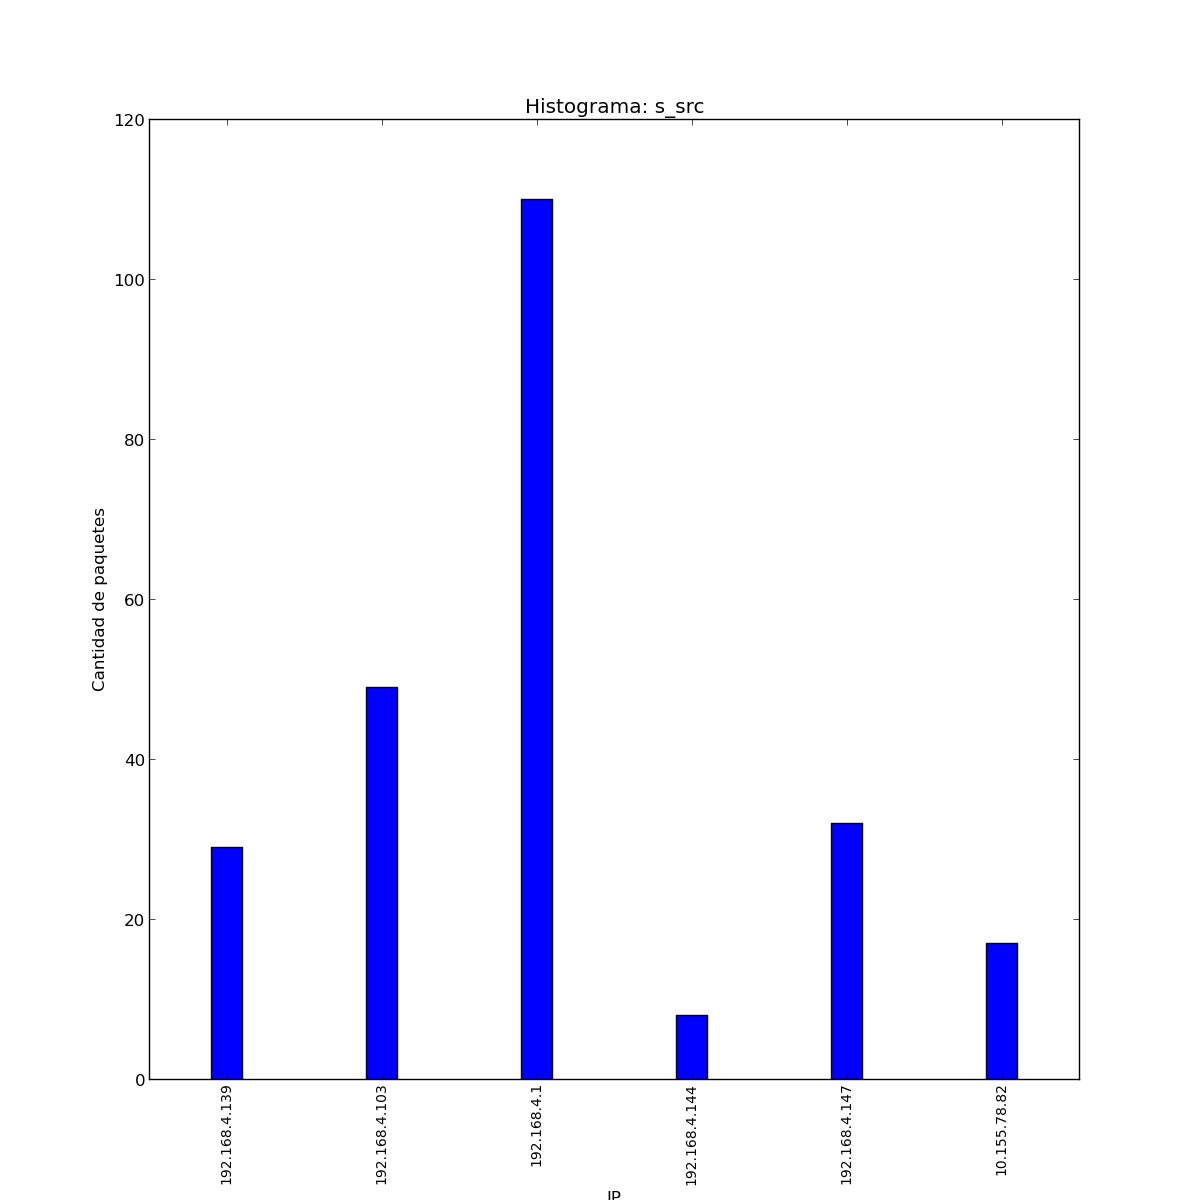
\includegraphics[width=\linewidth]{../imgs/prueba_laburo-ips_s_src_hist.png}
     \caption{Medición Honeywell}\label{fig:Honeywell-src-hist}
   \end{minipage}
  \hfill
   \begin{minipage}{0.5\linewidth}
     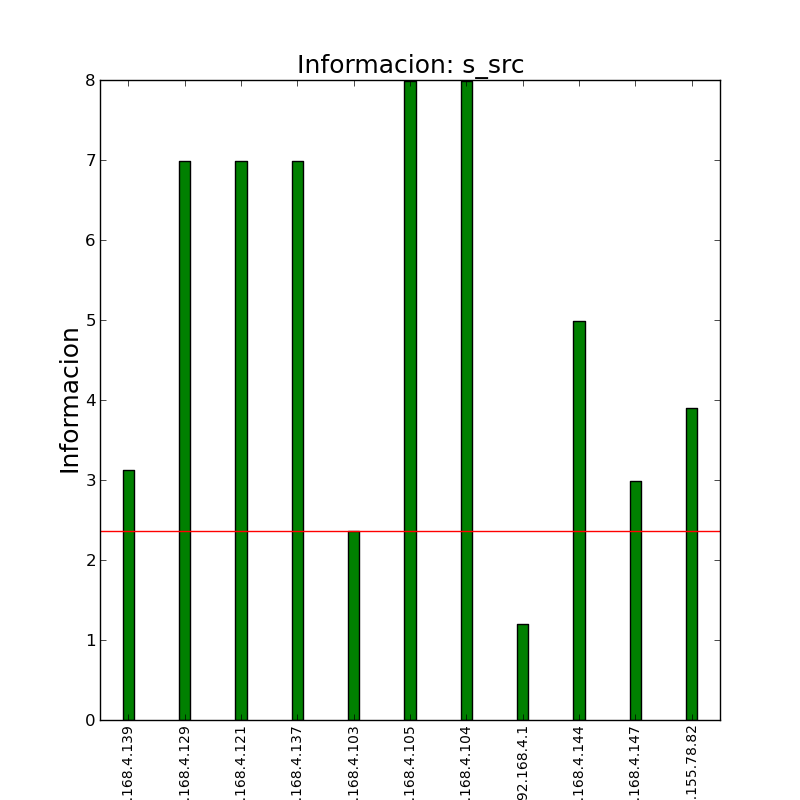
\includegraphics[width=\linewidth]{../imgs/prueba_laburo-ips_s_src_info.png}
     \caption{Medición Honeywell}\label{fig:Honeywell-src-	info}
   \end{minipage}
 \end{figure}

\subsection{Red Laboratorios DC}

\subsubsection{Descripción y topología de la red}

Realizamos una captura en la red Wi-Fi \emph{Entrepiso-DC}, disponible desde los laboratorios del Depto. de Computación. La muestra fue tomada un lunes a las 17hs aproximadamente -horario típicamente de alto tráfico-, logrando un total de XX paquetes en MM minutos.

En el gráfico de la figura \ref{fig:entrepiso-dc-grafo} se presenta el grafo dirigido representando la red. En el mismo se observa una gran cantidad de nodos ligada al nodo con IP 10.1.200.197, y luego múltiples conjuntos pequeños de nodos conectados entre sí pero disconexos de la estructura mayoritaria.

\begin{figure}[H]
  \begin{center}
    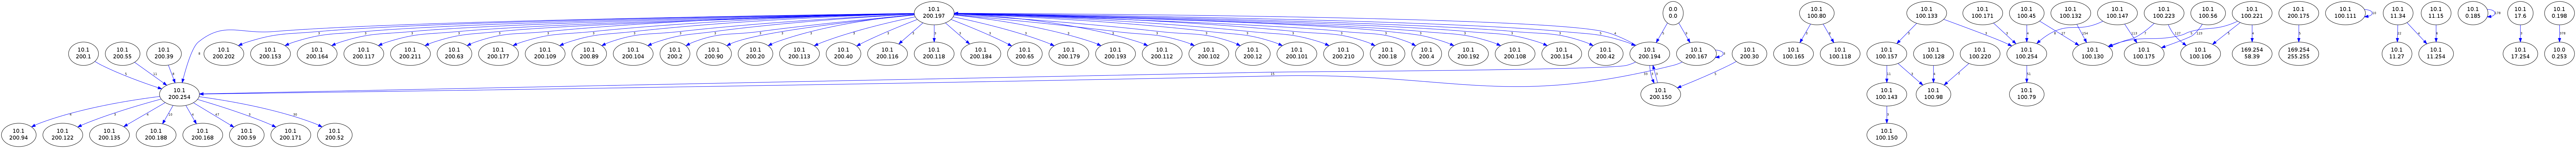
\includegraphics[width=0.8\linewidth]{../imgs/entrepiso-dc-ips_red.png}
    \caption{Grafo mostrando la topología de la red \emph{Entrepiso-DC}.}
    \label{fig:entrepiso-dc-grafo}
  \end{center}
\end{figure}

\subsubsection{Fuente: $S_{dst}$}

\begin{figure}[H]
  \begin{minipage}{0.48\linewidth}
    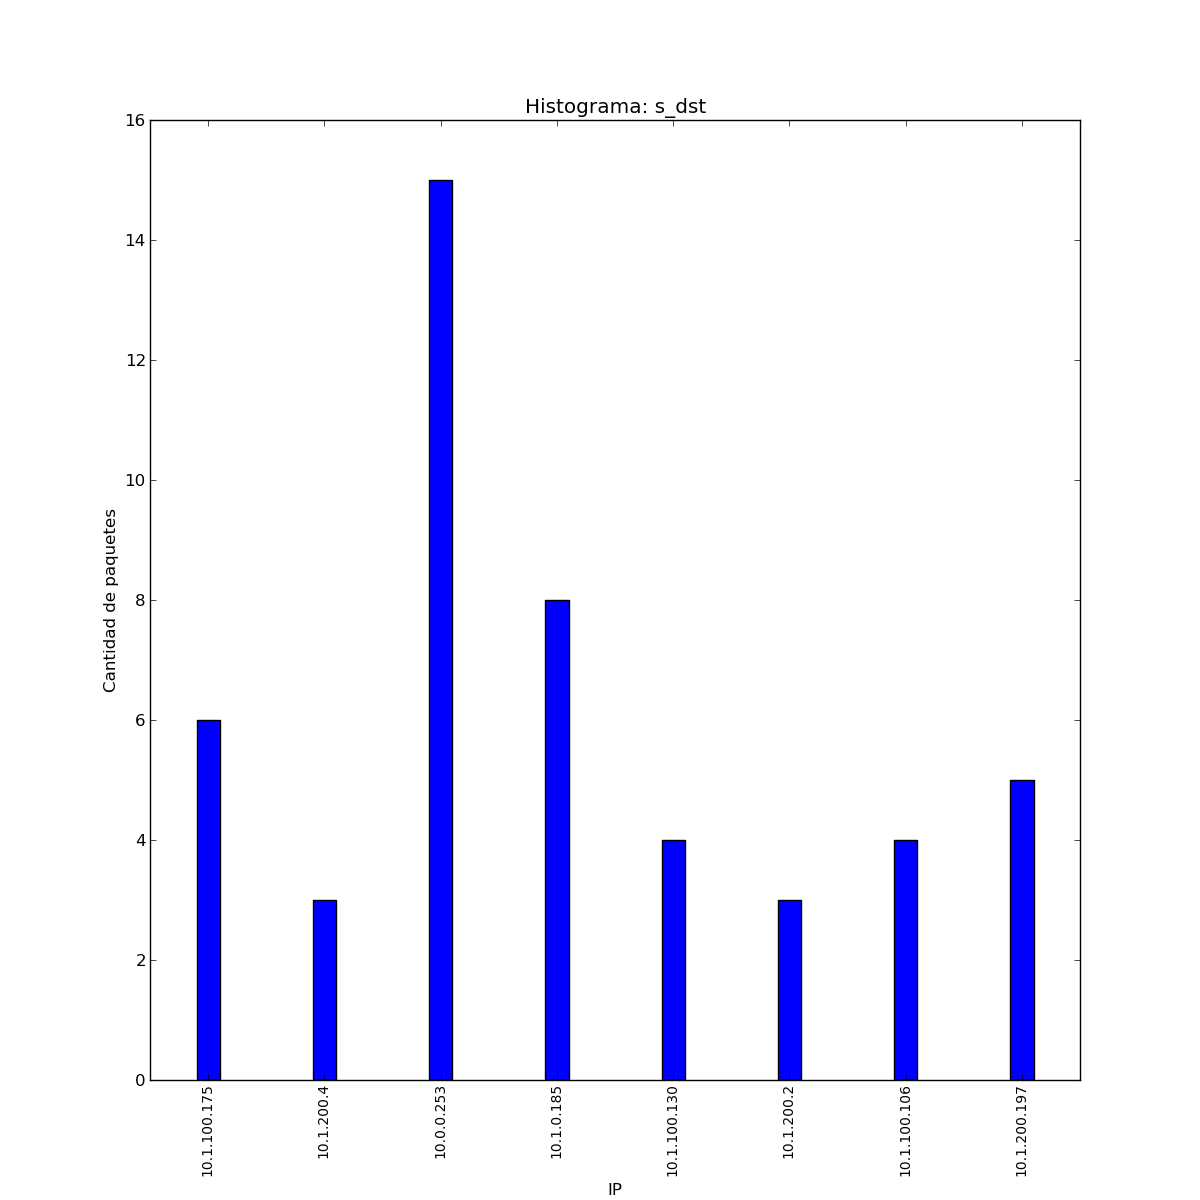
\includegraphics[width=\linewidth]{../imgs/entrepiso-dc-ips_s_dst_hist.png}
    \caption{Histograma de la serie de paquetes s\_dst de la red \emph{Entrepiso-DC}.}
    \label{fig:histograma-entrepiso-dc-s-dst}
  \end{minipage}
\hfill
  \begin{minipage}{0.48\linewidth}
    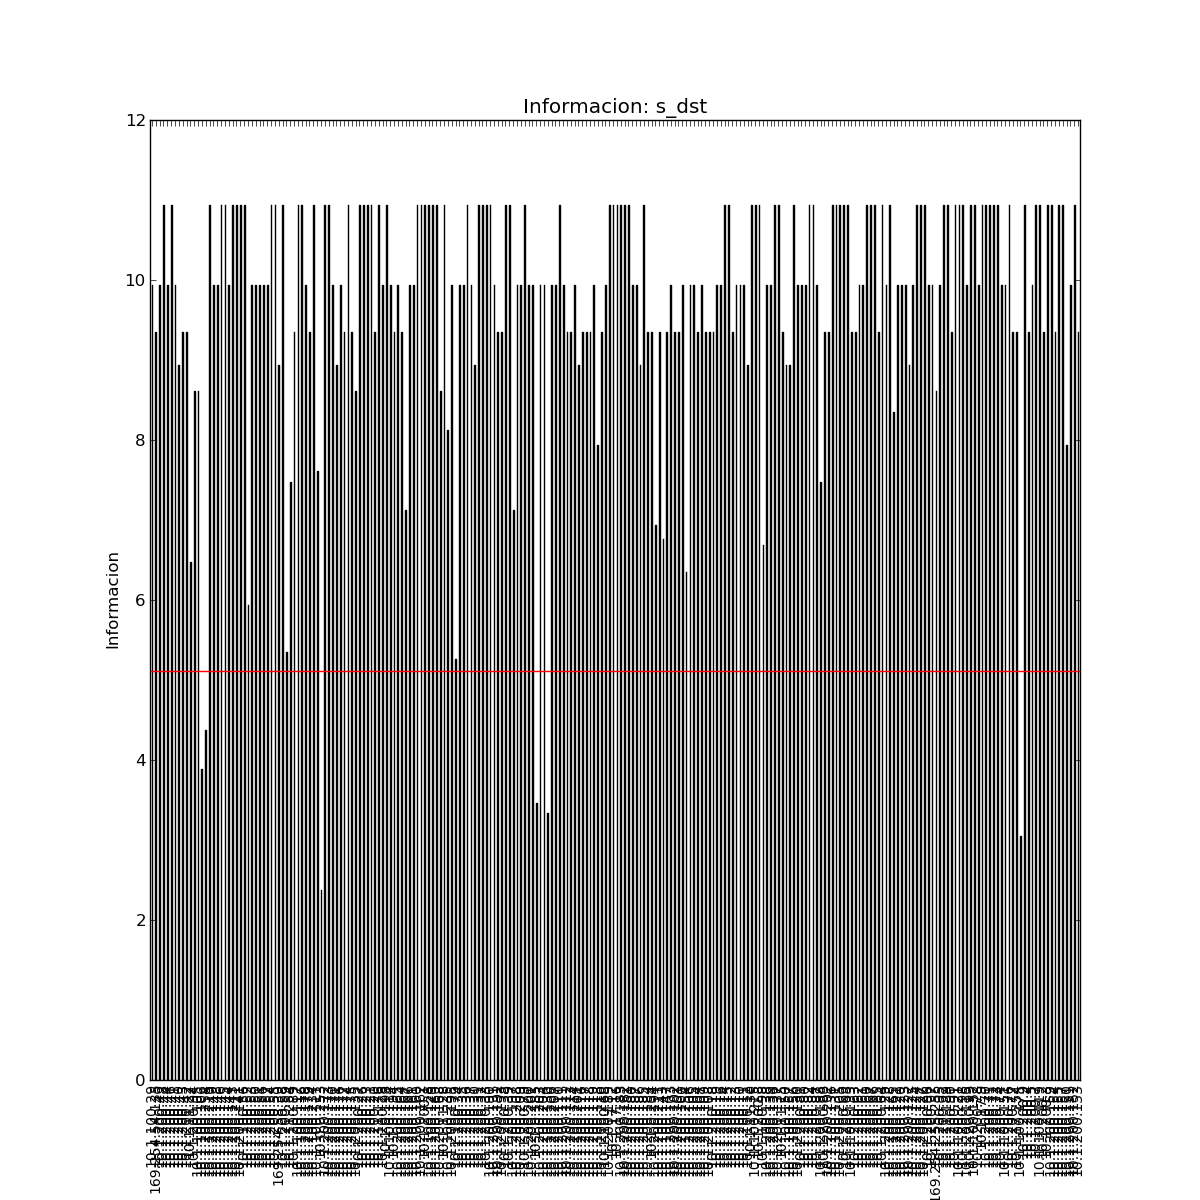
\includegraphics[width=\linewidth]{../imgs/entrepiso-dc-ips_s_dst_info.png}
    \caption{Gráfico de cantidad de información para cada IP s\_dst de la red \emph{Entrepiso-DC}.}
    \label{fig:informacion-entrepiso-dc-s-dst}
  \end{minipage}
\end{figure}

entropía total

\subsubsection{Fuente: $S_{src}$}

\begin{figure}[H]
  \begin{minipage}{0.48\linewidth}
    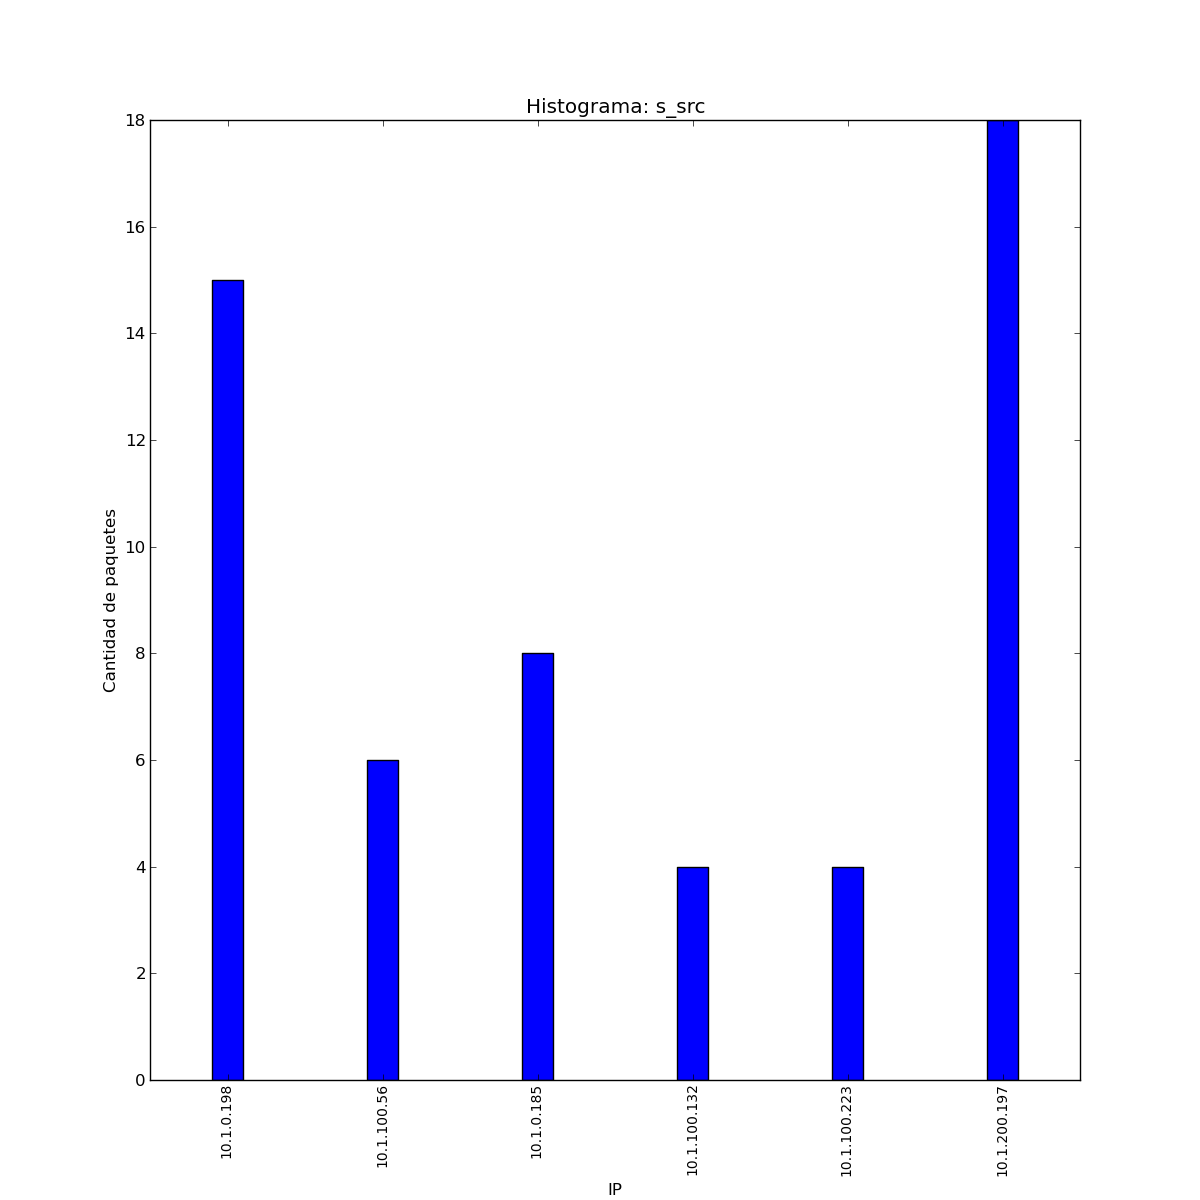
\includegraphics[width=\linewidth]{../imgs/entrepiso-dc-ips_s_src_hist.png}
    \caption{Histograma de la serie de paquetes s\_src de la red \emph{Entrepiso-DC}.}
    \label{fig:histograma-entrepiso-dc-s-src}
  \end{minipage}
\hfill
  \begin{minipage}{0.48\linewidth}
    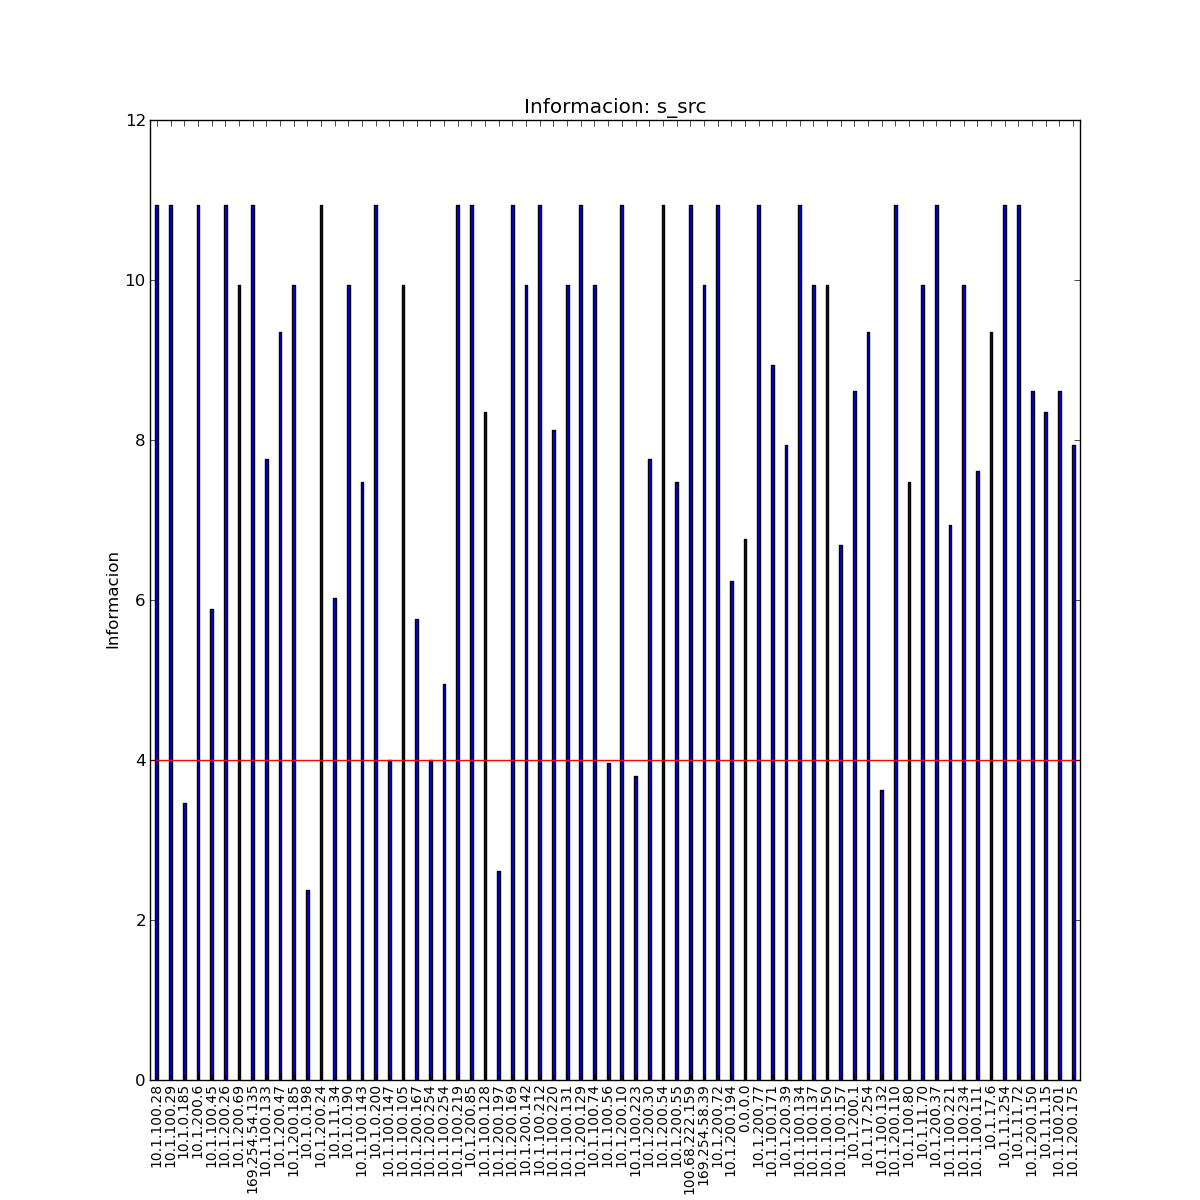
\includegraphics[width=\linewidth]{../imgs/entrepiso-dc-ips_s_src_info.png}
    \caption{Gráfico de cantidad de información para cada IP s\_src de la red \emph{Entrepiso-DC}.}
    \label{fig:informacion-entrepiso-dc-s-src}
  \end{minipage}
\end{figure}

entropía total

\subsubsection{Discusión}

cualquier cosa interesante sobre este caso en particular

\subsection{Red hogareña}

\subsubsection{Descripción}
Para nuestro último experimento, capturamos el tráfico de la LAN de un integrante de nuestro grupo. Medimos el Miércoles 17 de Septiembre a las 00:00 utilizando la red Wi-Fi. El tiempo de medición fue de aproximadamente 40 minutos, y capturamos aproximadamente 20 paquetes.

\subsubsection{Topología de la red}

\begin{figure}[H]
  \begin{center}
    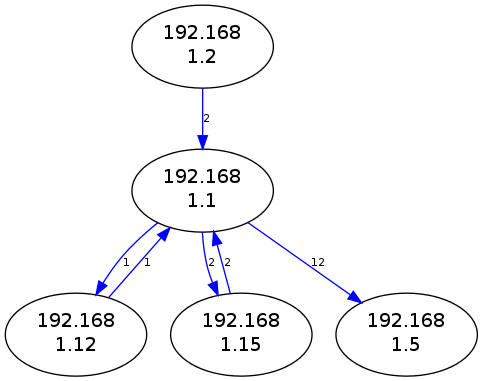
\includegraphics[width=\linewidth/2]{../imgs/pruebaFede-ips_red.png}
    \label{fig:FedeGrafo}
    \caption{Grafo de LAN hogareña}
  \end{center}
\end{figure}

\subsubsection{Fuente: $S_{dst}$}

$\bullet$ Entropía de la fuente: 1.49046857073

\begin{figure}[H]
  \begin{minipage}{0.5\linewidth}
    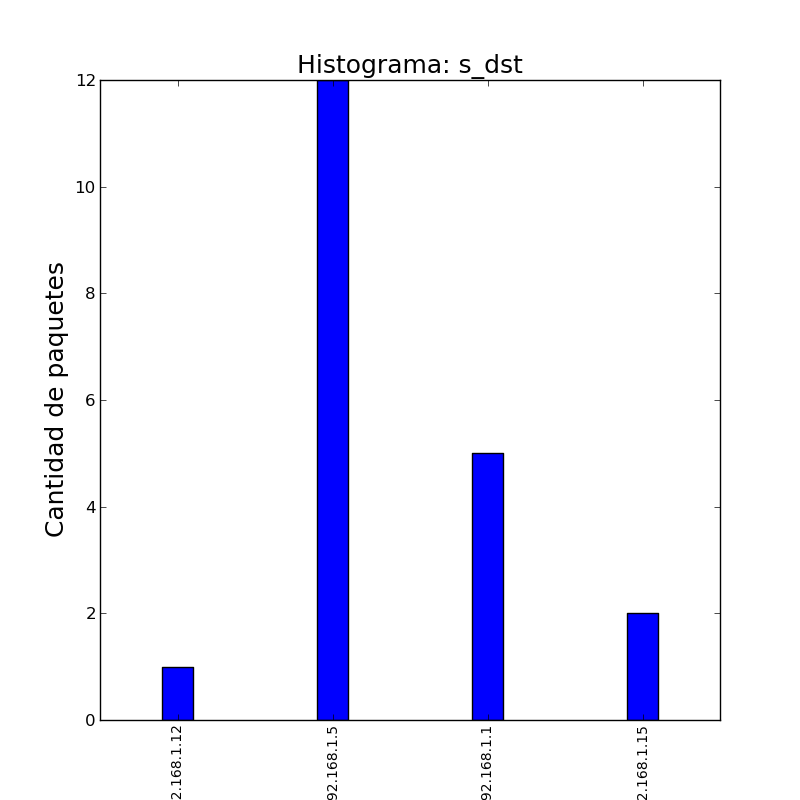
\includegraphics[width=\linewidth]{../imgs/pruebaFede-ips_s_dst_hist.png}
    \caption{Histograma de $S_{dst}$}\label{fig:Fede-dst-hist}
  \end{minipage}
\hfill
  \begin{minipage}{0.5\linewidth}
    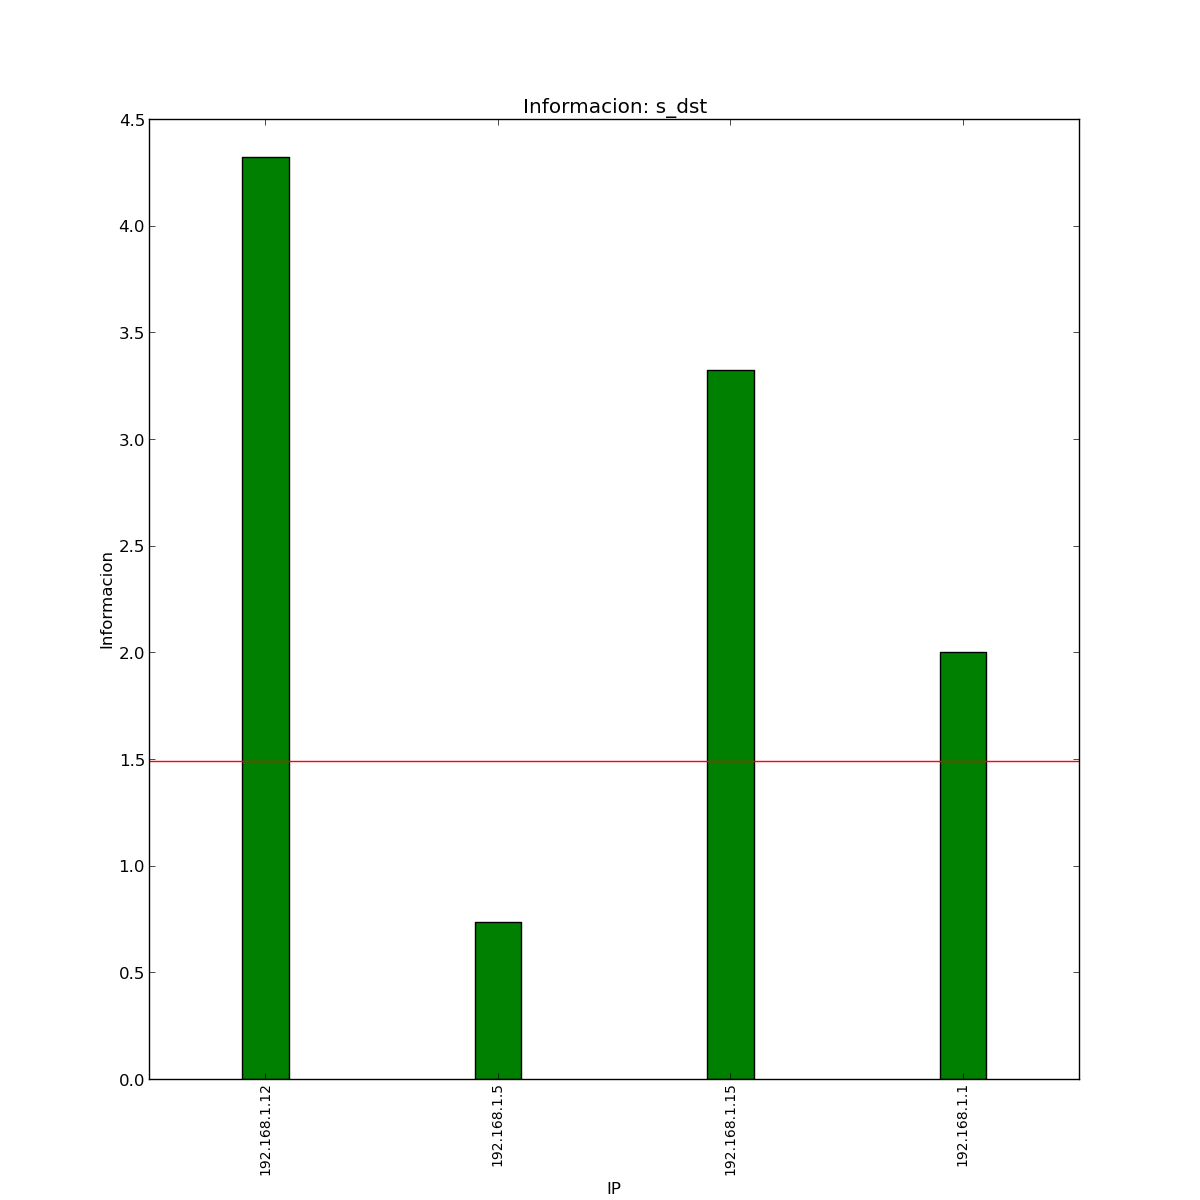
\includegraphics[width=\linewidth]{../imgs/pruebaFede-ips_s_dst_info.png}
    \caption{Informacion de $S_{dst}$}\label{fig:Fede-dst-info}
  \end{minipage}
\end{figure}

\subsubsection{Fuente: $S_{src}$}

$\bullet$ Entropía de la fuente: 1.19176014818

\begin{figure}[H]
  \begin{minipage}{0.5\linewidth}
    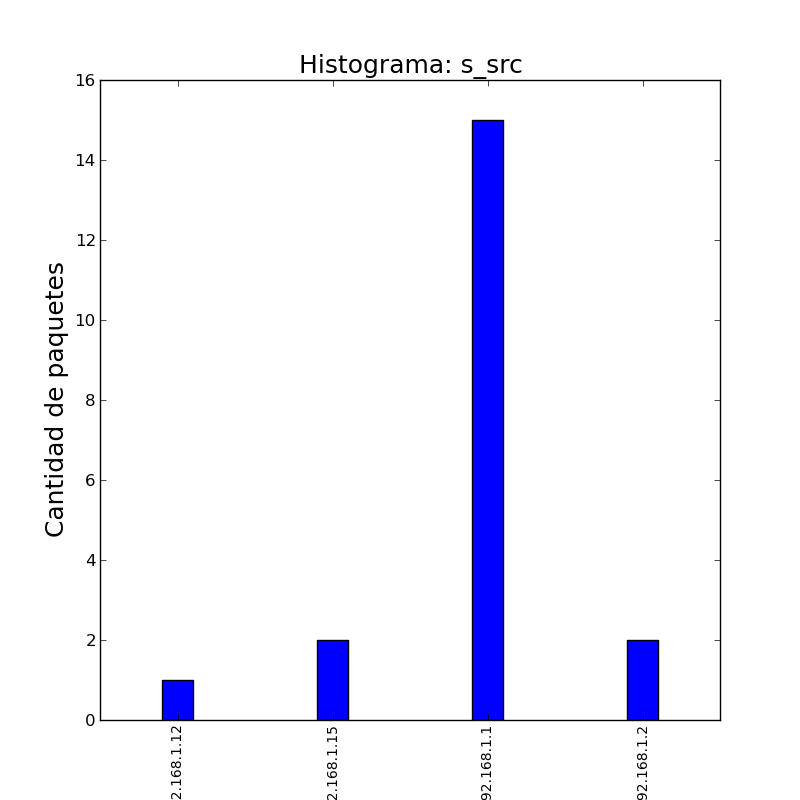
\includegraphics[width=\linewidth]{../imgs/pruebaFede-ips_s_src_hist.png}
    \caption{Histograma de $S_{src}$}\label{fig:Fede-src-hist}
  \end{minipage}
\hfill
  \begin{minipage}{0.5\linewidth}
    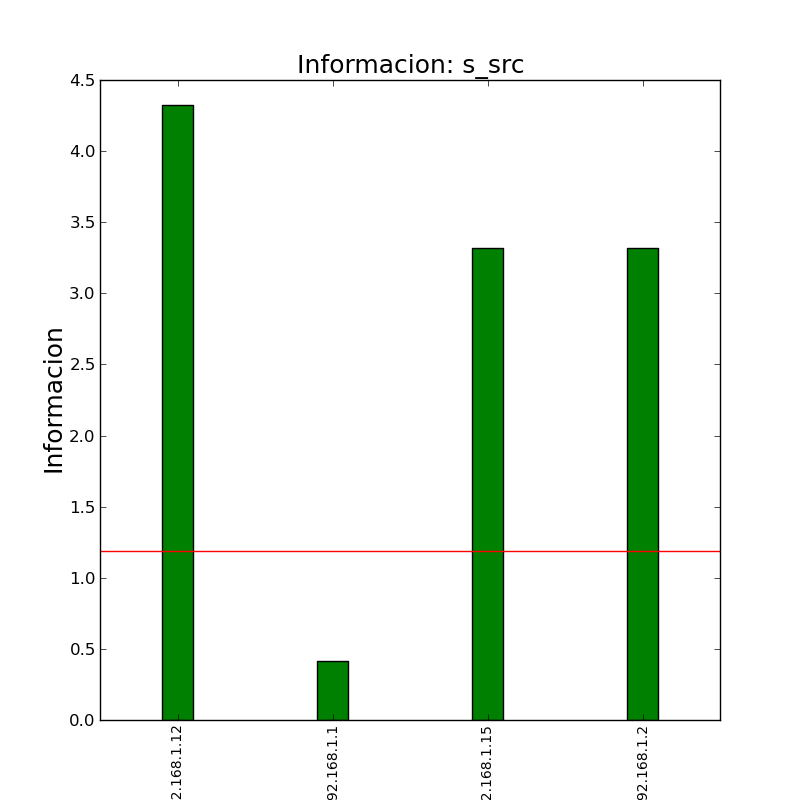
\includegraphics[width=\linewidth]{../imgs/pruebaFede-ips_s_src_info.png}
    \caption{Informacion de $S_{src}$}\label{fig:Fede-src-info}
  \end{minipage}
\end{figure}

\subsubsection{Discusión}

cualquier cosa interesante sobre este caso en particular

\section{Discusión general}

\section{Conclusión}
Como conclusión, queremos recalcar que por lo general los routers son nodos distinguidos en las LANs a las que pertenecen. Esto se mantiene, ya sea una red pública o privada.

Como pudimos ver en los experimentos, creemos que es importante saber que esto no necesariamente siempre es así. En el caso de Ciudad Universitaria, el servidor local era un nodo distinguido.

Para finalizar, en este trabajo práctico aprendimos que LA AMISTAD RESUELVE TODOS LOS PROBLEMAS.
\end{document}	